\documentclass[aspectratio=169]{beamer}
\usepackage[utf8]{inputenc}
%\usepackage[sfmath]{kpfonts}
\usepackage{helvet}
\usepackage[euler]{textgreek}
%\usepackage{lmodern}
\usepackage{siunitx}
\usepackage{tikz}

\usepackage{xcolor}
\usepackage{hyperref}

\hypersetup{
  colorlinks,
  citecolor=cyan,
  linkcolor=blue}


\usetheme{Madrid}
%\usecolortheme{default}

\usepackage[backend=biber]{biblatex}
%\bibliography{refs.bib}
\addbibresource{refs.bib}

%------------------------------------------------------------
%This block of code defines the information to appear in the
%Title page
\title[Microcontroller architecture] %optional
{Microcontroller architecture}

\subtitle{ISA and Microarchitecture}

\author{Daniel Giovanni Martínez Sandoval} 

\institute[CUCEI - UDG]
{
  \textsc{
    \textbf{Universidad de Guadalajara}\\
    {\tiny Centro Universitario de Ciencias Exactas e Ingenierías}
  }
}

\date[September 2024] % (optional)
{\footnotesize I7266 - Programación de Sistemas Embebidos - 2024B }

\titlegraphic { 
  \begin{tikzpicture}[overlay,remember picture]
  \node[right=-2.5cm] at (current page.345){
    
\includegraphics[height=20mm]{assets/logo_udg_color.eps}
  };
  \end{tikzpicture}
}
%\logo{
\includegraphics[height=15mm]{logo_udg_color.eps}}

%End of title page configuration block
%------------------------------------------------------------



%------------------------------------------------------------
%The next block of commands puts the table of contents at the 
%beginning of each section and highlights the current section:

\AtBeginSection[]
{
  \begin{frame}
    \frametitle{Table of Contents}
    \tableofcontents[currentsection]
\end{frame}
}
%------------------------------------------------------------


\begin{document}

%The next statement creates the title page.
\frame{\titlepage}


%---------------------------------------------------------
%This block of code is for the table of contents after
%the title page
\begin{frame}
\frametitle{Table of Contents}
\tableofcontents
\end{frame}
%---------------------------------------------------------


\section{Computer architecture}
\subsection{What is an architecture?}
\subsubsection{Definition}
%---------------------------------------------------------
\begin{frame}
  \frametitle{Definition of architecture}
  ``Architecture'' is a broad term in computer science, but we will stick to this definition: \pause
  \begin{block}{Architecture}
    Architecture describes the internal organization of a computer in an abstract way; that is, it defines the capabilities of the computer and its programming model.\cite{clements} \pause
  \end{block}
  Basically, it is an abstraction that outlines how a computer's hardware components interact and work together to process data. Of course it is important. But why?
  \end{frame}
%---------------------------------------------------------

\subsubsection{Importance}
%---------------------------------------------------------
\begin{frame}
  \frametitle{Importance of architecture}
  In embedded systems, architecture plays a crucial role because these systems are mostly designed for specific tasks rather than general-purpose computing. Some things to take into account when choosing an architecture are:\pause
  \begin{itemize}
    \item <2-> \textbf{Power consumption:} Many embedded systems operate on battery power. A microcontroller packed with features but with a high current consumption is not always feasible for battery-operated systems. 
    \item <3-> \textbf{Cost and size:} Choosing a microcontroller with just enough features to develop the intended functionality is key to saving money, but also in some cases the size, which in turn also reduces the cost.
    \item <4-> \textbf{Performance and memory:} Depending on the application, some devices might only run certain OS which is targeted for a specific arquitechture, or maybe they need to be compatible with external memory. 
  \end{itemize}
\end{frame}
%---------------------------------------------------------

%---------------------------------------------------------
\begin{frame}
  \frametitle{Importance of architecture (cont.)}
  So, just like buying any other thing, when buying a microcontroller to design an embedded system, you should take into account the size, your budget, the style, among many other things. But the thing with architecture in computer science and embedded systems is that saying ``architecture'' is really, really broad. \pause \\[5mm]
  Why? you may ask... Well, in the beginning we had very simple circuits compared to those nowadays. We also had one way to program them: 1's and '0s. But today we have a huge variety of variables, even with circuits themselves, since we're not limited to Microcontrollers(\textmu Cs or MCUs) and Microprocessors(\textmu Ps), we also have Digital Signal Processors (DSPs), Field Programmable Gate Arrays (FPGAs), System-on-Chips (SoCs), and Application Specific Integrated Circuits (ASICS).  
\end{frame}
%---------------------------------------------------------

%---------------------------------------------------------
\begin{frame}
  \frametitle{Different kinds of architectures}
  I said that architecture is a broad term, and is not only because of the current complexity of computational systems, but also because of the many variants of architecture or the many ways that we can organize components inside a microcontroller in order to understand its functionality. \pause

  So, let us explore some different kinds of architectures.
\end{frame}
%---------------------------------------------------------

\subsubsection{ISA}
%---------------------------------------------------------
\begin{frame}
  \frametitle{ISAs}
    \begin{block}{Instruction Set Architecture}
      An Instruction Set Architecture (ISA) is part of the abstract model of a computer that defines how the CPU is controlled by the software. The ISA acts as an interface between the hardware and the software, specifying both what the processor is capable of doing as well as how it gets done. \cite{ISA} \pause
    \end{block} 
    The ISA provides the only way through which a user is able to interact with the hardware. It can be viewed as a programmer's manual because it is the portion of the machine that's visible to the assembly language programmer, the compiler writer, and the application programmer. 
  \end{frame}
%---------------------------------------------------------

%---------------------------------------------------------
\begin{frame}
  \frametitle{ISAs (cont.)}
  Some popular ISAs are: \pause
  \begin{itemize}
    \item <2-> \textbf{ARM:} Used in smartphones. Based in RISC.
    \item <3-> \textbf{x86:} Used in desktop and laptop computers. Is a CISC.
    \item <4-> \textbf{RISC-V:} An \textit{open-source} ISA.
    \item <5-> \textbf{MIPS:} Based in RISC and used in many network systems.
    \item <6-> \textbf{AVR:} 8-bit RISC, which we will explore and use in this course.
  \end{itemize}
\end{frame}
%---------------------------------------------------------

\subsubsection{Microarchitecture}
%---------------------------------------------------------
\begin{frame}
  \frametitle{Microarchitecture}
  \begin{block}{Microarchitecture}
    Microarchitecture is the implementation of the ISA in hardware. It defines how a processor's internal components are organized and interact to execute the instructions described by the ISA.   
  \end{block}
  ISAs can be executed in different implementations of hardware, so, a microarchitecture (or \textmu arch) is the description of that exact thing. 
\end{frame}
%---------------------------------------------------------

%---------------------------------------------------------
% \begin{frame}
%   \frametitle{Microarchitecture (cont.)}
%   begin{columns}[T]
%     \begin{column}{.5\textwidth}
%      \begin{block}{Microarchitectures are usually represented as diagrams that describe the interconnections of the various microarchitectural elements of the machine, which may include gates, registers, arithmetic ALUs and even larger elements. These diagrams generally also include the buses.}
% % Your text here
%     \end{block}
%     \end{column}
%     \begin{column}{.5\textwidth}
%     \begin{block}{Your image}
% % Your image included here
%     \captionsetup{justification=centering}
% 			\includegraphics{328p_uarch.png} % Imagen
% 			\caption{Pie de imagen 1} % Pie de imagen
% 			\label{img:1} % Etiqueta
%     \end{block}
%     \end{column}
%   \end{columns}
% \end{frame}
%---------------------------------------------------------

%---------------------------------------------------------
\begin{frame}
  \frametitle{Microarchitecture (cont.)}
  Microarchitectures are usually represented as diagrams that describe the interconnections of the various microarchitectural elements of the machine, which may include gates, registers, arithmetic ALUs and even larger elements. These diagrams generally also include the buses. 
\end{frame}
%---------------------------------------------------------

\subsubsection{Memory architexture}
%---------------------------------------------------------
\begin{frame}
  \frametitle{Memory hierarchy}
  Memory hierarchy architecture refers to the structured levels of memory in a computer system, from the fastest (but smallest) to the slowest (but largest) storage. The hierarchy helps balance speed, cost, and capacity. In a typical modern microcontroller we can usually find:
  \begin{itemize}
    \item <2-> Registers
    \item <3-> Cache 
    \item <4-> RAM 
    \item <5-> Flash 
    \item <6-> EEPROM 
  \end{itemize}
\end{frame}
%---------------------------------------------------------

%---------------------------------------------------------
\begin{frame}
  \frametitle{Memory hierarchy (cont.)}
  \begin{itemize}
    \item <1-> \textbf{Registers}: The fastest type of memory located within the CPU, used to store temporary data and intermediate values during computation.
    \item <2-> \textbf{Cache}: These are small storage regions used for frequently accessed information. Can be located inside or really close to the CPU and it is really fast. Generally, we find three levels of cache:
    \begin{itemize}
      \item <3-> \textbf{L1}: The fastest, and also the smallest. Usually found inside the CPU. Stores recently used instructions or data that are most likely to be requested again soon.
      \item <3-> \textbf{L2 \& L3}: Typically external. Store additional information that may be needed by the processor in order to run efficiently; they are slightly slower than Level 1 but still provide quick access when necessary.
    \end{itemize}
  \end{itemize}
\end{frame}
%---------------------------------------------------------

%---------------------------------------------------------
\begin{frame}
  \frametitle{Memory hierarchy (cont.)}
  \begin{itemize}
    \item <1-> \textbf{Flash}: A type of non-volatile memory in which data persists even after the power is turned off, it is cheap, small and reliable.
    \item <2-> \textbf{EEPROM}: Electrically Erasable Programmable Read-Only Memory. Offers faster byte-level writes and erases, making it suitable for applications with occasional updates (e.g., configuration settings). Still, flash provides higher storage density, better endurance through wear-leveling, and is more cost-effective for larger storage capacities and applications that require frequent data updates.
  \end{itemize}
\end{frame}
%---------------------------------------------------------

\subsubsection{Examples}
%---------------------------------------------------------
\begin{frame}
  \frametitle{Real architectures}
  We have studied some basics about architectures, so... \pause
  \begin{block}
    How do architectures really look?
  \end{block}
\end{frame}
%---------------------------------------------------------

%---------------------------------------------------------
\begin{frame}{Von-Neumann Architecture}
  \begin{itemize}
      \item <1-> Single memory space: Program instructions and data share the same memory.
      \item <2-> Unified bus: A single bus is used for transferring both instructions and data between memory and the CPU.
      \item <3-> Execution bottleneck: Since instructions and data share the same bus, the system can experience delays (known as the Von Neumann bottleneck) when fetching instructions and data alternately.
  \end{itemize}
\end{frame}
%---------------------------------------------------------

%---------------------------------------------------------
\begin{frame}{Von-Neumann Architecture}
\begin{center}
  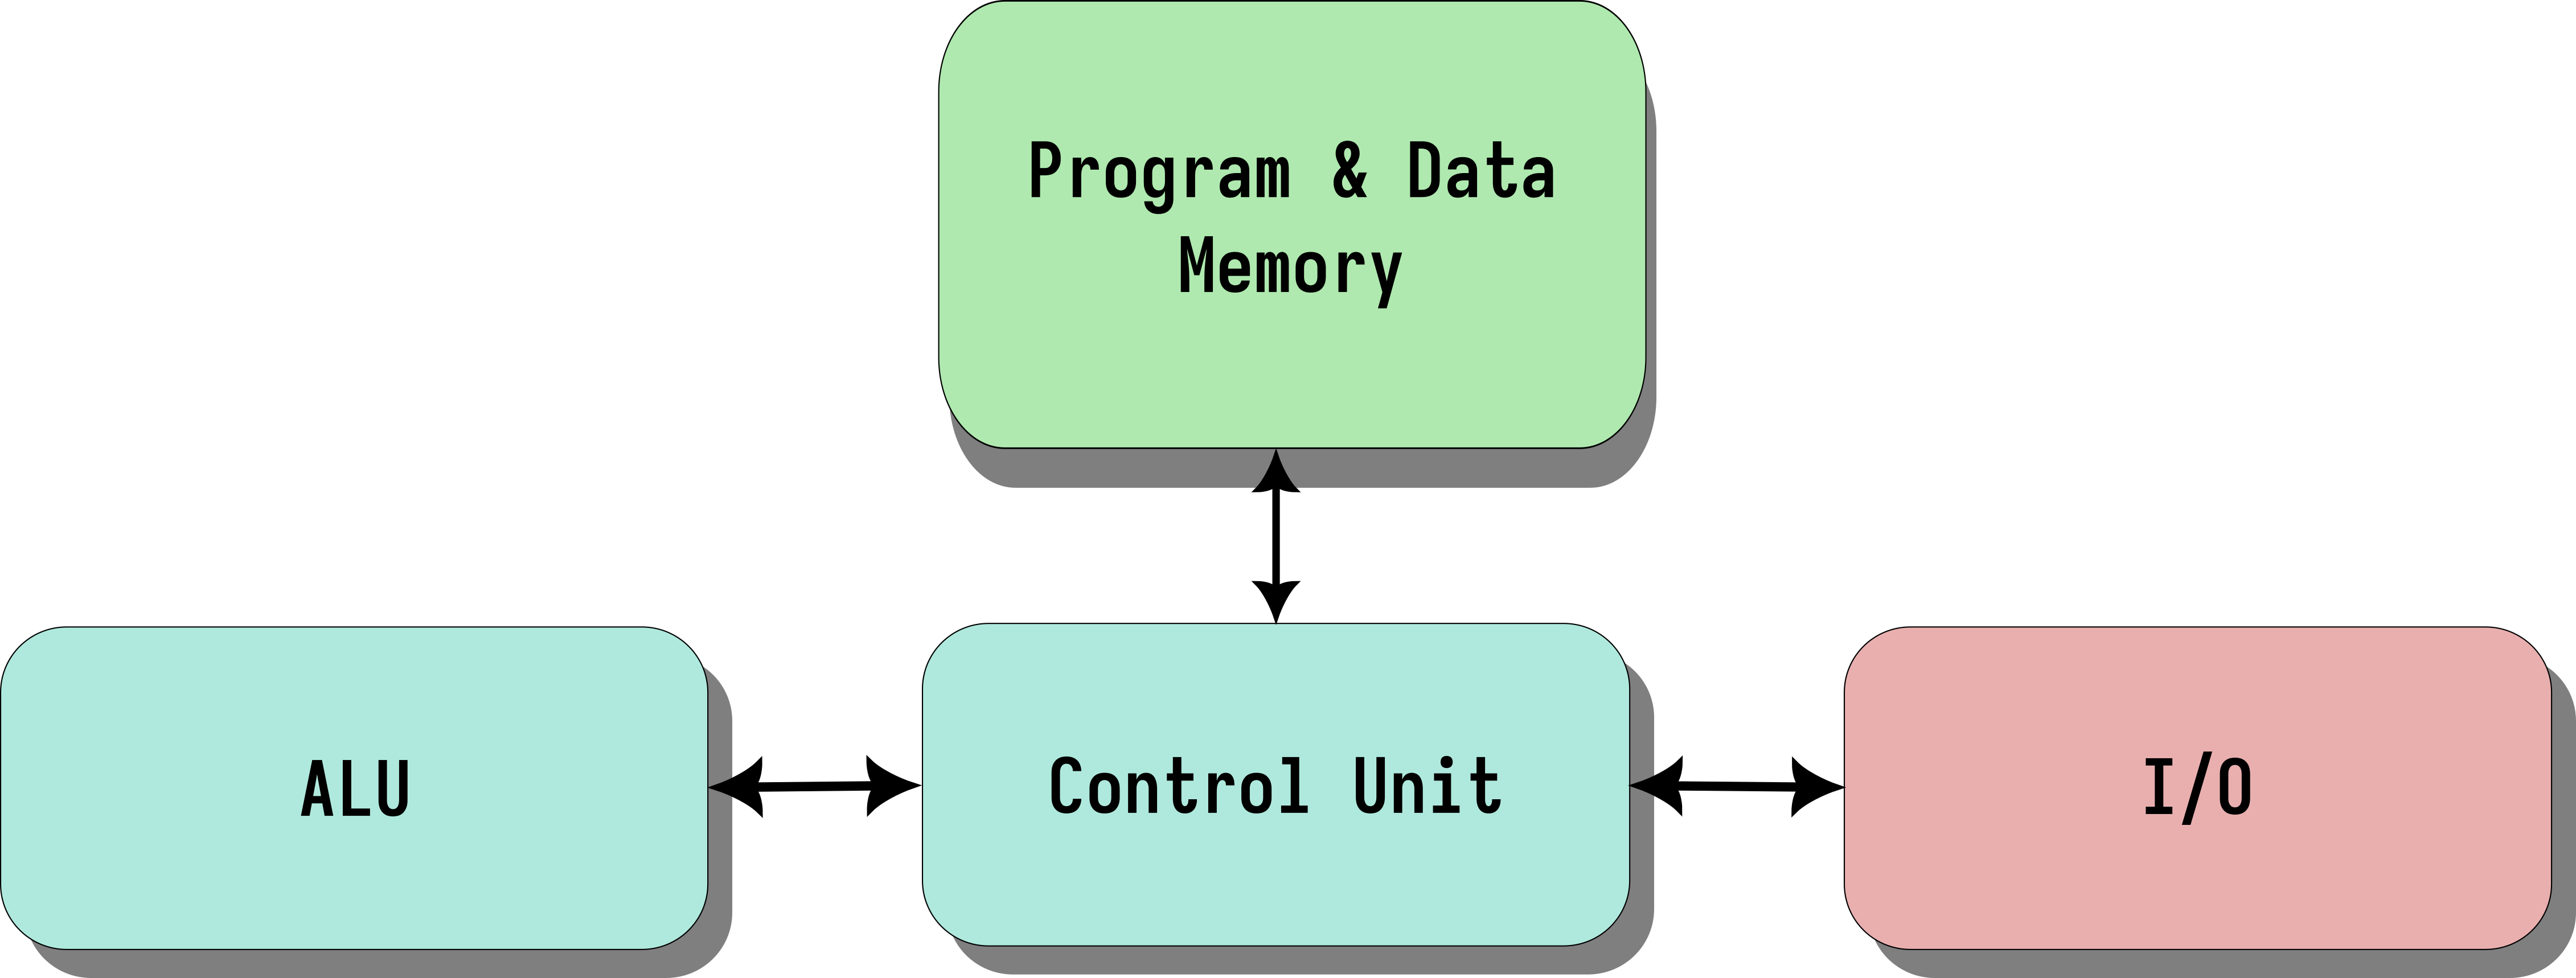
\includegraphics[width=0.6\textwidth]{assets/von_neumann_arch.png}  
\end{center}
\end{frame}
%---------------------------------------------------------

%---------------------------------------------------------
\begin{frame}{Harvard Architecture}
  \begin{itemize}
      \item <1-> Separated memory spaces: instruction memory (Flash) and data memory (SRAM).
      \item <2-> Separate buses: The CPU can fetch instructions and access data simultaneously because it uses two separate buses for instruction and data transfer.
      \item <3-> Faster execution: This separation reduces the bottleneck since fetching instructions does not interfere with data access.
  \end{itemize}
\end{frame}
%---------------------------------------------------------

%---------------------------------------------------------
\begin{frame}{Harvard Architecture}
\begin{center}
  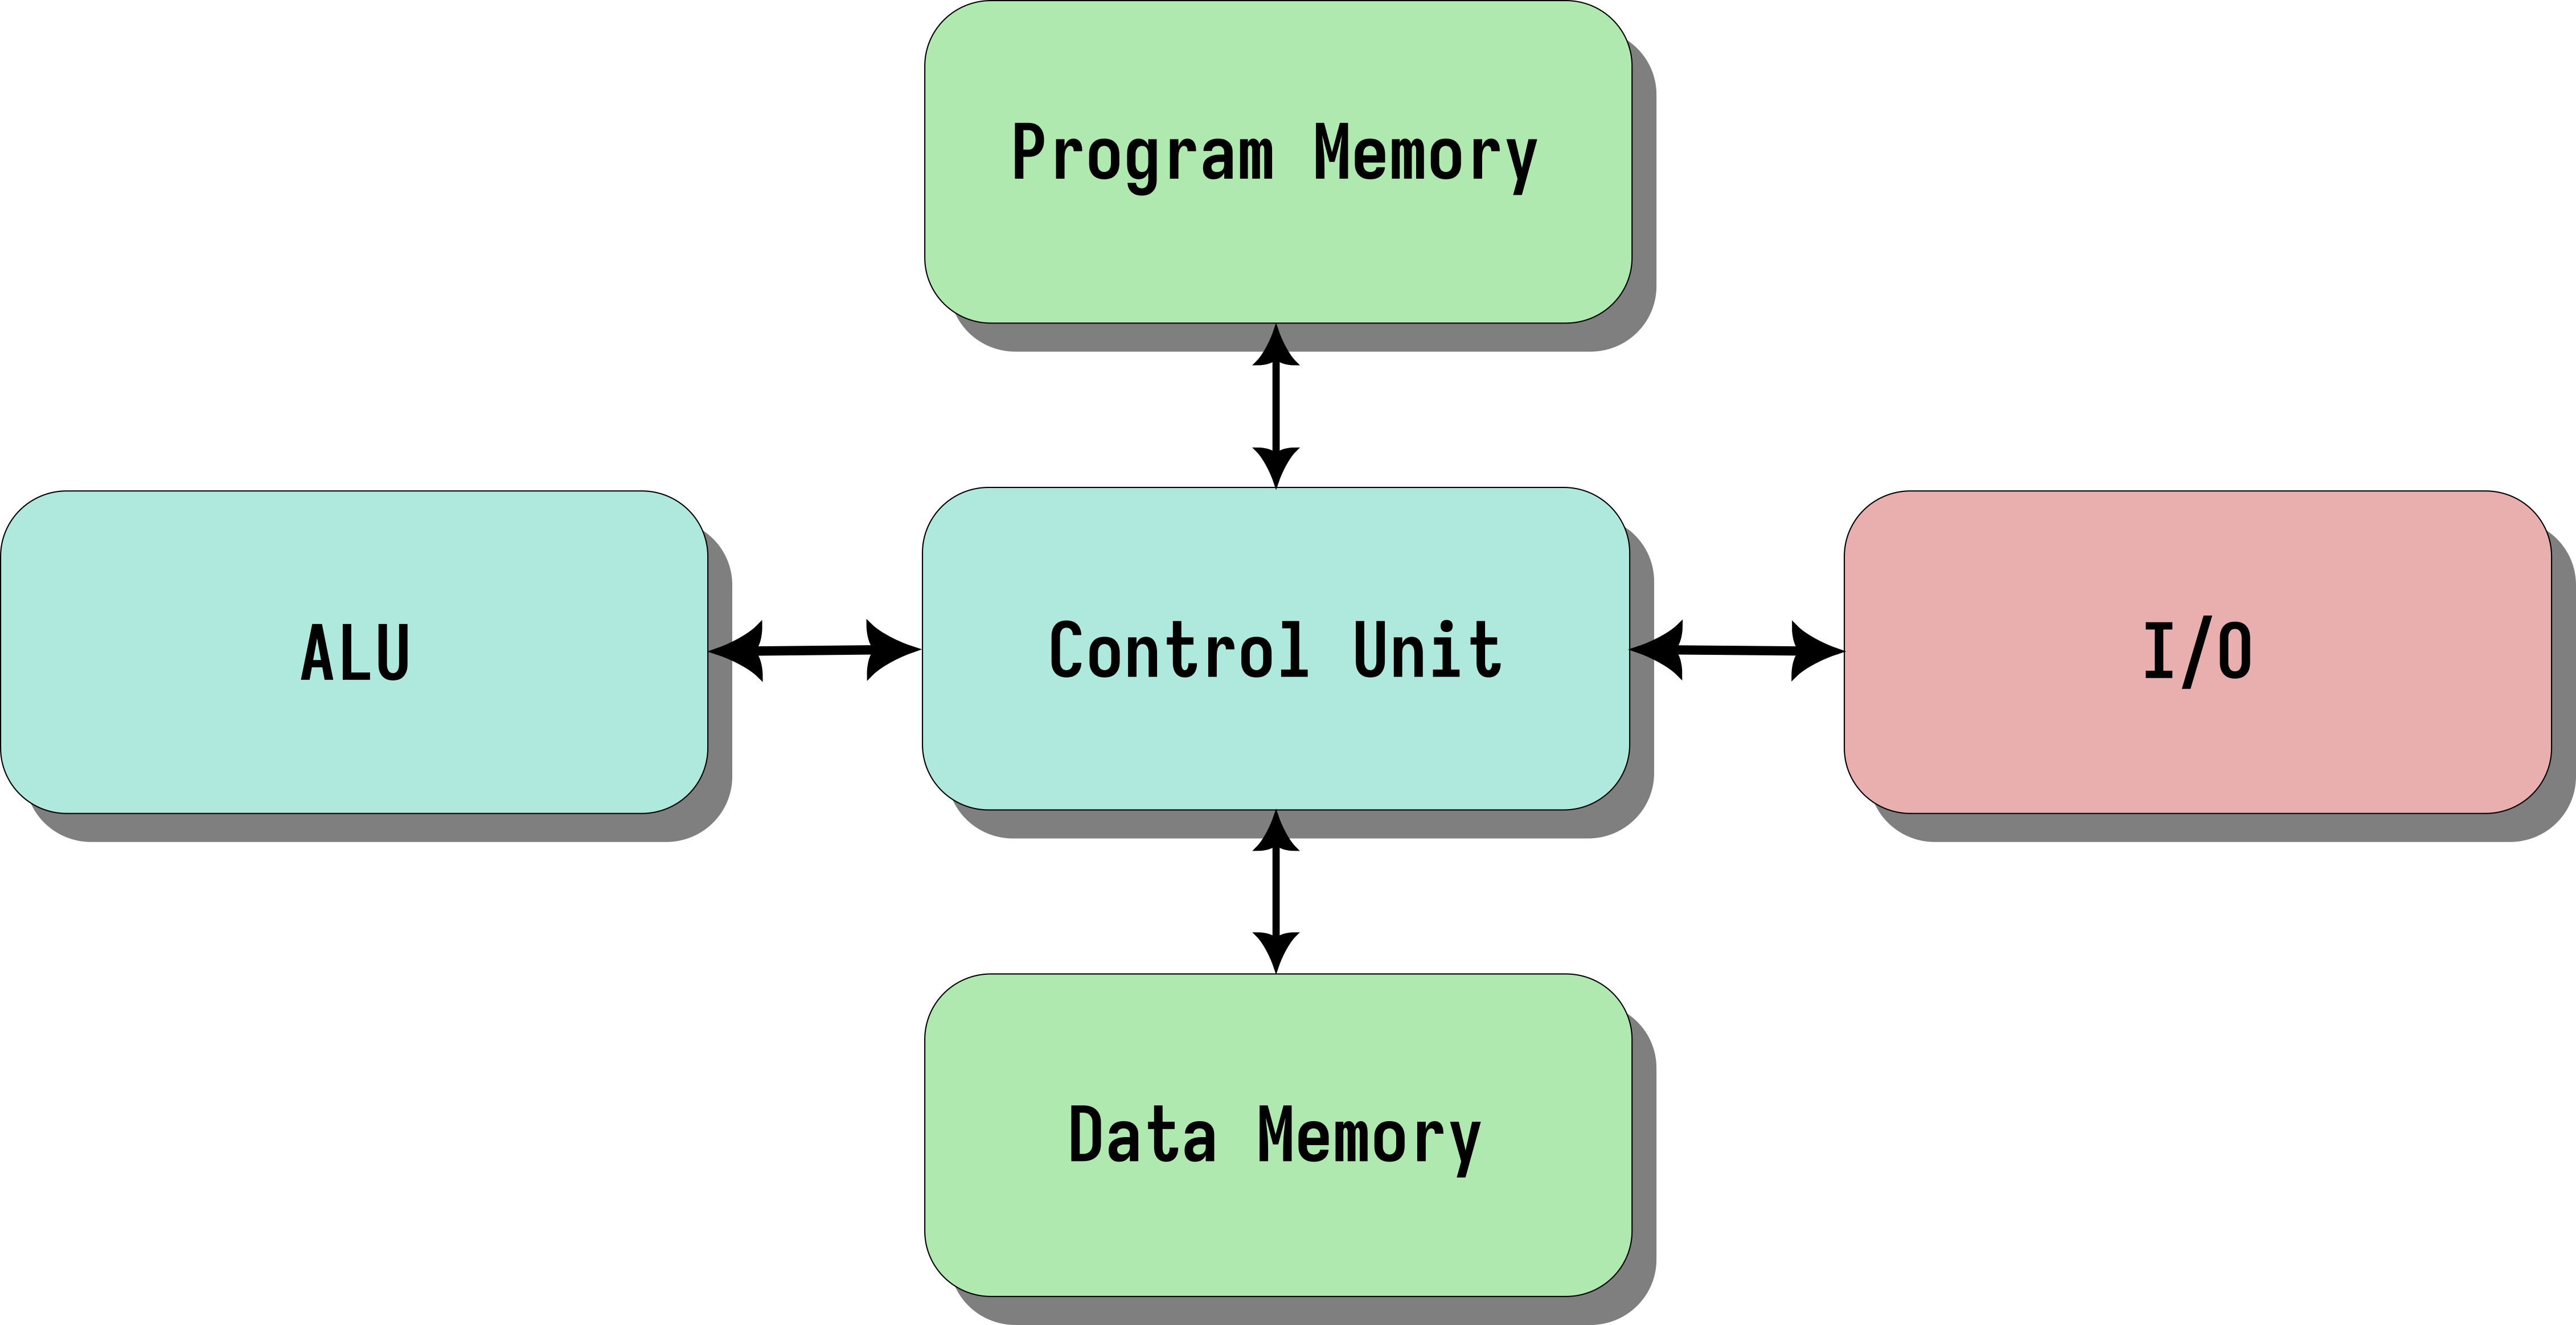
\includegraphics[width=0.6\textwidth]{assets/harvard_arch.png}  
\end{center}
\end{frame}
%---------------------------------------------------------

%---------------------------------------------------------
\begin{frame}
  \frametitle{ATmega328P architecture}
  \centering
  \includegraphics[height=0.9\textheight]{assets/328p_uarch.png}
\end{frame}
%---------------------------------------------------------

\subsection{The instruction cycle}
\subsubsection{Definition}
%---------------------------------------------------------
\begin{frame}{The instruction cycle}
  The instruction cycle is the process by which a microprocessor (or microcontroller) achieves the execution of each instruction. It is the fundamental operation that allow these devices to perform tasks. It constists of the following steps:
  \begin{enumerate}
        \item <2-> Fetch: Retrieving the instruction from memory.
        \item <3-> Decode: Interpreting what the instruction is meant to do.
        \item <4-> Execute: Performing the operation specified by the instruction.
  \end{enumerate}
  Each step consists of multiple other steps. But to understand these steps we should also understand what instructions and microinstructions are.
\end{frame}
%---------------------------------------------------------

\subsubsection{Microinstrucions}
%---------------------------------------------------------
\begin{frame}{Instructions and microinstructions}
  A CPU is capable of executing the instructions that the ISA describes and the \textmu arch provides hardware for. 
  There might be instructions, for example, a multiplication instruction, which may involve multiple steps, like to move the data to multiply to a register close to the ALU, and then operate and then move the result to another register. This is: a single ISA instruction might be comprised of multiple microinstructions, however, microinstructions are internal to CPU and they are out of our reach, but they still play a big role in microcontroller architectures.
\end{frame}
%---------------------------------------------------------

\subsubsection{The instruction cycle}
%---------------------------------------------------------
\begin{frame}{The instruction cycle (cont.)}
  \textbf{\large Fetch:}
  \begin{enumerate}
    \item <2-> The \textit{progam counter} (PC) is previously loaded with the address of the next instruction to be fetched.
    \item <3-> The address is copied to the \textit{memory address register} (MAR)
    \item <4-> The data from the MAR is sent across the address bus, and the contents of the address are accessed.
    \item <5-> The data from that location in memory is sent down the data bus to the \textit{memory data register} (MDR). 
    \item <6-> There is now an instruction to decode and the PC increments.
  \end{enumerate}
\end{frame}
%---------------------------------------------------------

%---------------------------------------------------------
\begin{frame}{The instruction cycle (cont.)}
  \textbf{\large Decode:}
  \begin{enumerate}
        \item <2-> The instruction is placed into the \textit{current instruction register} (CIR).
        \item <3-> The data is split into the \textit{opcode} and the \textit{operand}.
        \item <4-> Those are sent to the \textit{control unit} (CU).
  \end{enumerate}
\end{frame}
%---------------------------------------------------------

%---------------------------------------------------------
\begin{frame}{The instruction cycle (cont.)}
  \textbf{\large Execute:}
  \begin{enumerate}
        \item <2-> This part is really dependant on the instruction we are executing.
        \item <3-> Maybe more data is read and then, processed.
        \item <4-> Then the ALU would do something with it.
        \item <5-> The result should be stored into a register.
        \item <6-> Other registers or flags might be afected and in turn, signal for the next instruction.
  \end{enumerate}
\end{frame}
%---------------------------------------------------------

\subsubsection{Examples}
%---------------------------------------------------------
\begin{frame}{RISC Architecture}
  \begin{itemize}
      \item <1-> Small, simple instruction set: RISC processors use a small set of simple instructions that can be executed quickly, usually in one clock cycle.
      \item <2-> Load/store architecture: Only load and store instructions can access memory, while other instructions operate on registers.
      \item <3-> Pipelining: RISC designs are highly pipelined, meaning multiple instructions can be processed simultaneously at different stages (fetch, decode, execute).
      \item <4-> Energy efficiency: Simple instructions and faster execution lead to more efficient use of power, which is critical for embedded systems.
  \end{itemize}
  % \begin{center}
  %     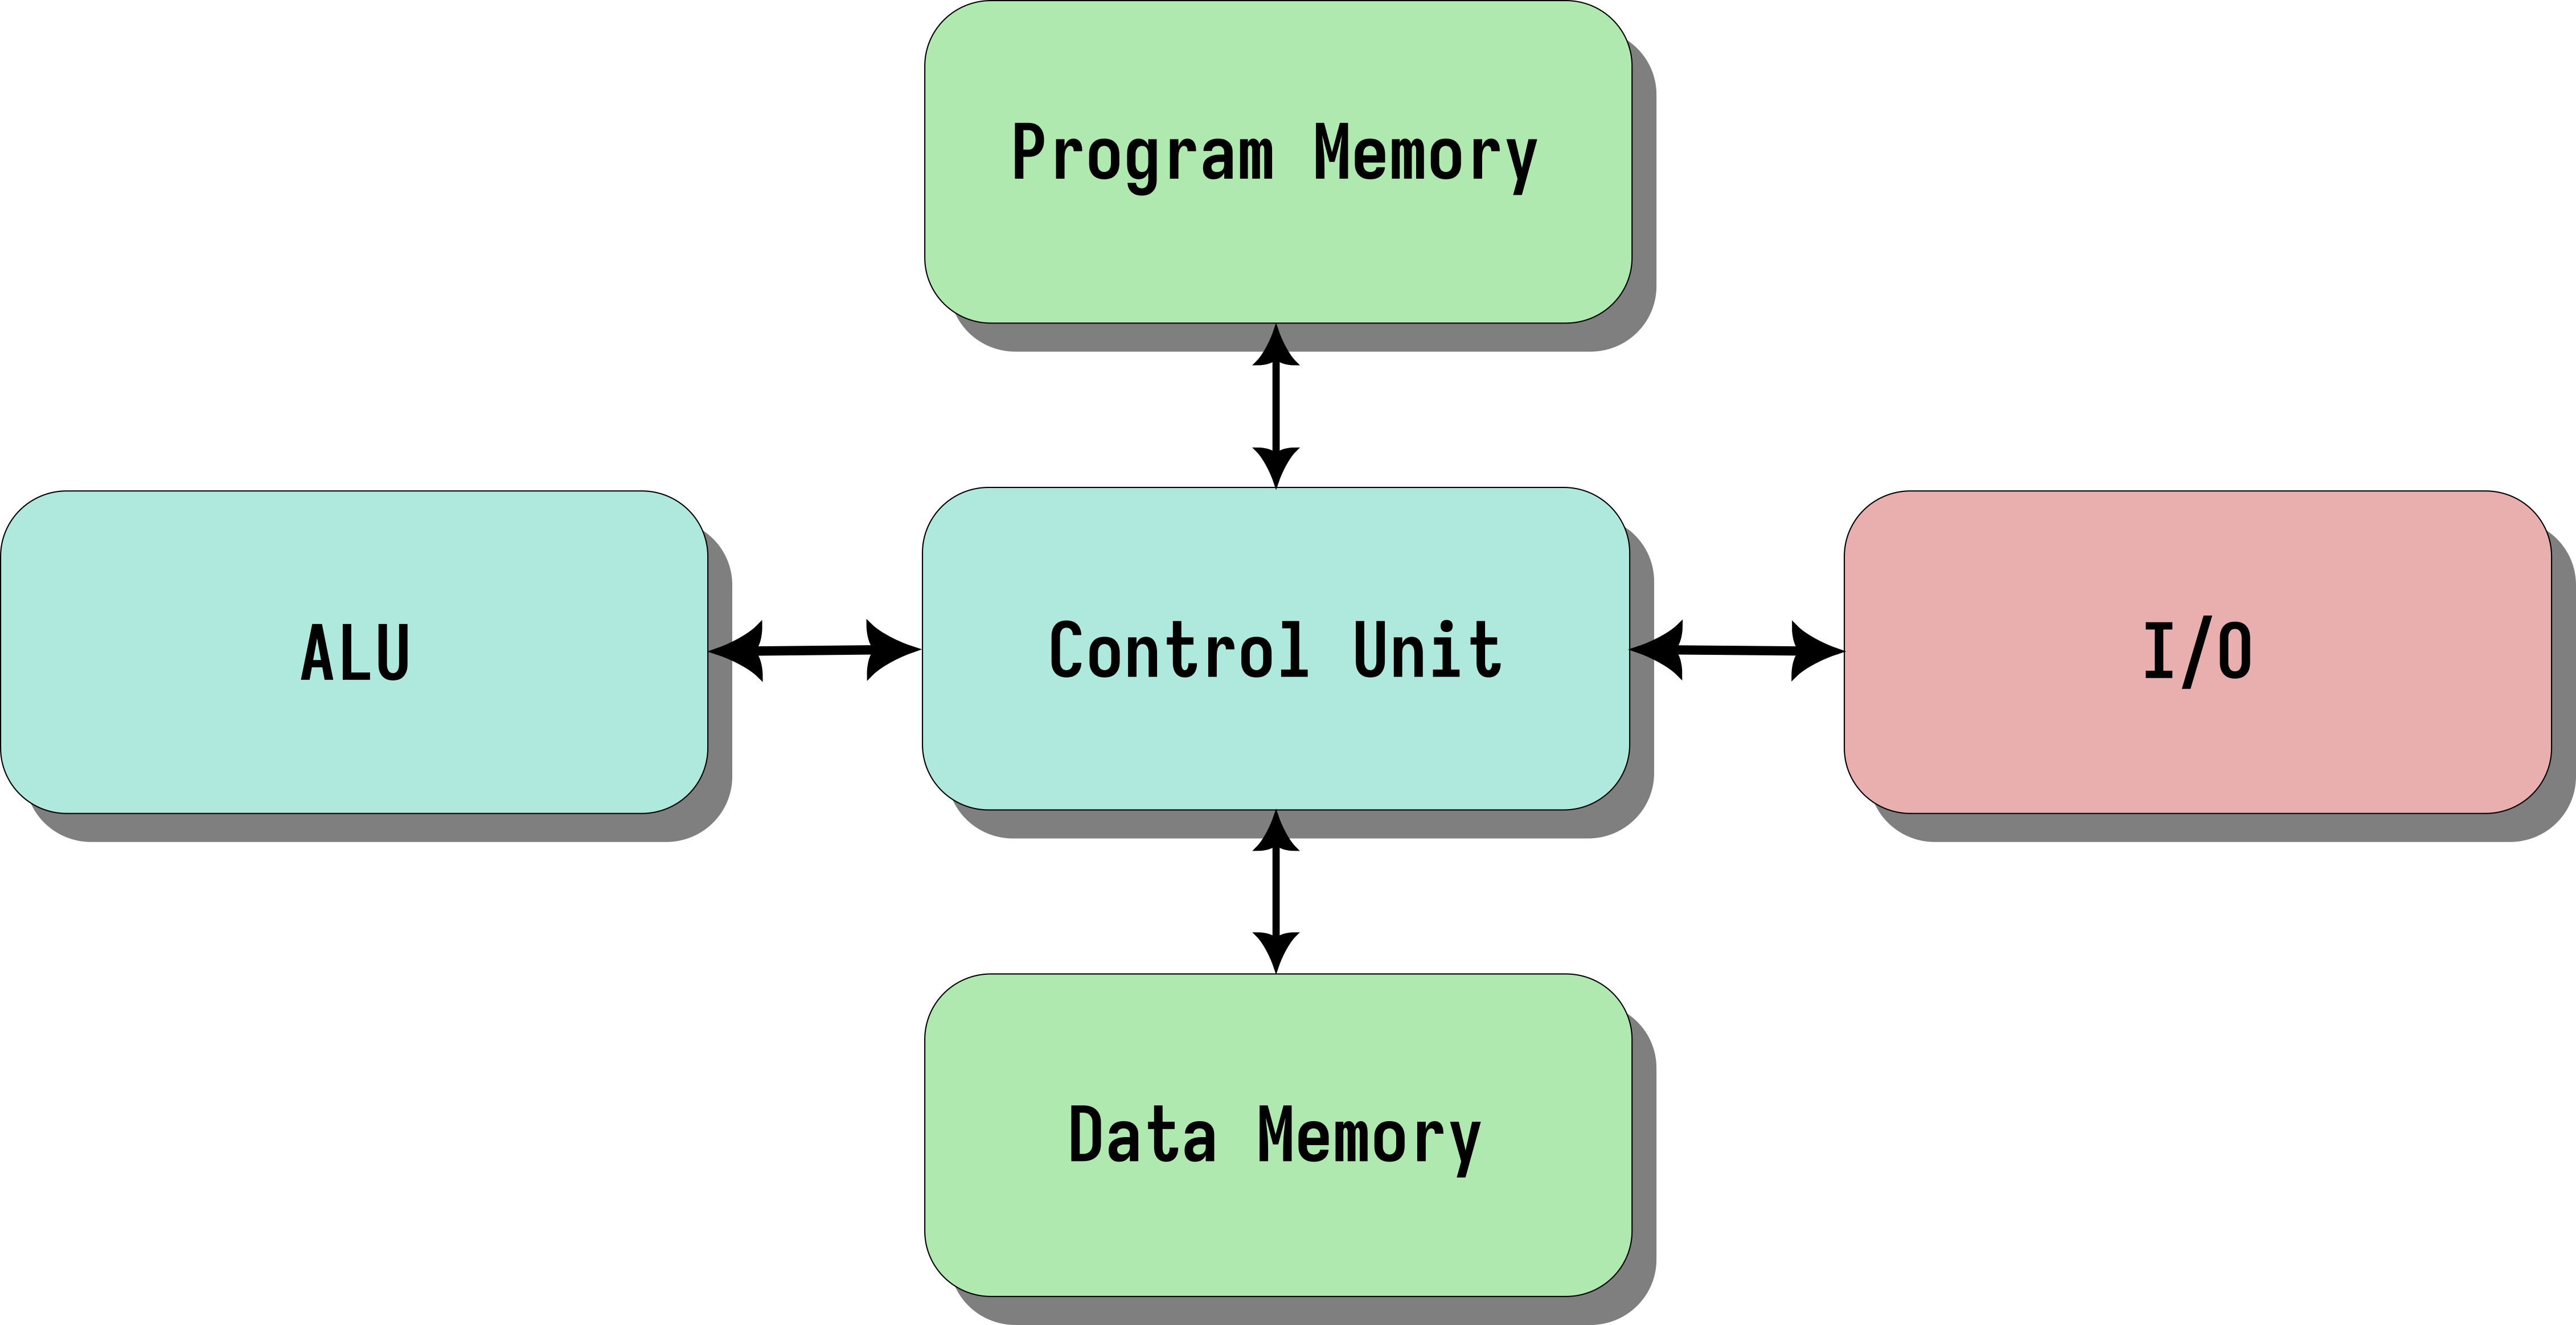
\includegraphics[width=0.6\textwidth]{assets/harvard_arch.png}  % Replace with actual image
  % \end{center}
\end{frame}
%---------------------------------------------------------

%---------------------------------------------------------
\begin{frame}{CISC Architecture}
    \begin{itemize}
        \item <1-> Large, complex instruction set: CISC processors have a large number of complex instructions, some of which can perform multiple tasks in a single instruction.
        \item <2-> Direct memory access: CISC instructions can directly operate on memory, reducing the need for multiple load/store instructions.
        \item <3-> Longer instruction execution time: Due to the complexity of CISC instructions, they generally take more clock cycles to execute than RISC instructions.
    \end{itemize}
    % \begin{center}
    %     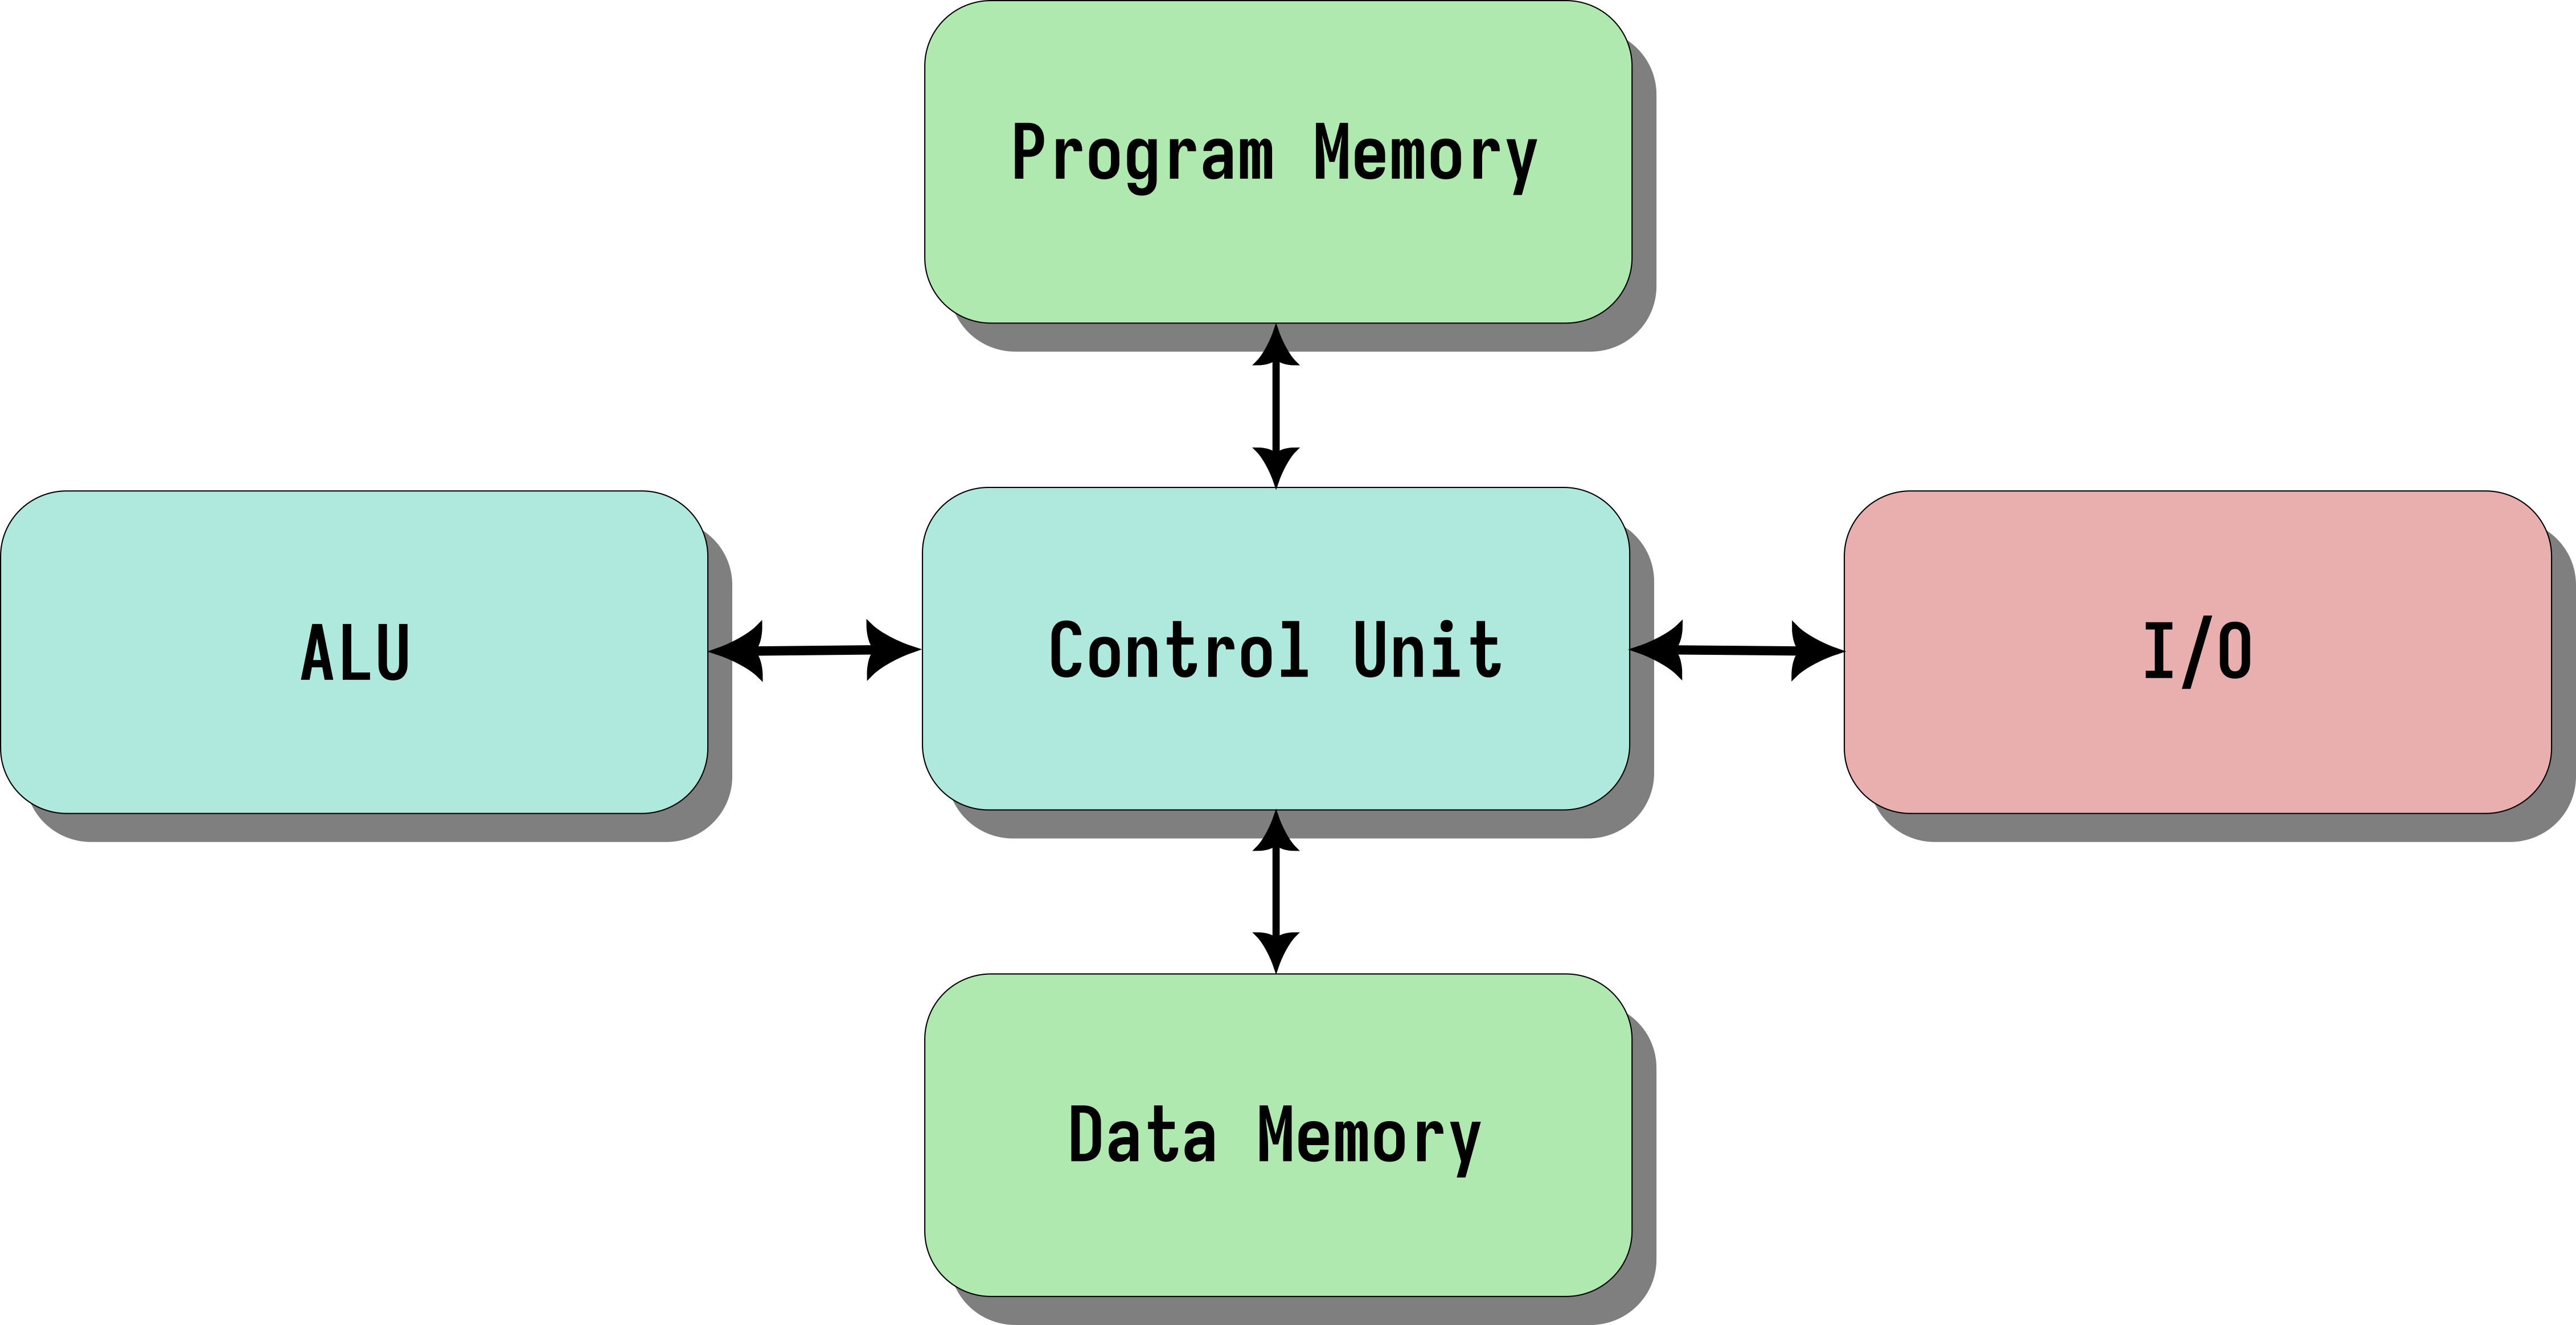
\includegraphics[width=0.6\textwidth]{assets/harvard_arch.png}  % Replace with actual image
    % \end{center}
\end{frame}
%---------------------------------------------------------

%---------------------------------------------------------
\begin{frame}
  \frametitle{ATmega328P architecture}
  \centering
  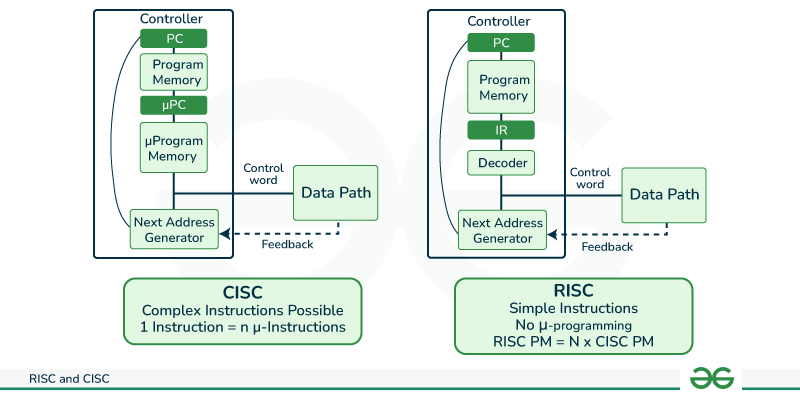
\includegraphics[height=0.9\textheight]{assets/RISC-and-CISC.png}
\end{frame}
%---------------------------------------------------------

%---------------------------------------------------------
\begin{frame}{Introduction to ATmega328P}
    \begin{itemize}
        \item <1-> ATmega328P is an 8-bit AVR microcontroller. (\textit{What does this mean?})
        \item <2-> It is widely used in Arduino boards (e.g., Arduino Uno).
        \item <3-> Features a RISC architecture with 32 general-purpose registers.
    \end{itemize}
\end{frame}
%---------------------------------------------------------

%---------------------------------------------------------
\begin{frame}{Core Features}
    \begin{itemize}
        \item <1-> \textbf{CPU}: 8-bit AVR with Harvard architecture.
        \item <2-> \textbf{Clock Speed}: Up to 20 MHz.
        \item <3-> \textbf{Flash Memory}: 32 KB for program storage.
        \item <4-> \textbf{SRAM}: 2 KB for data storage.
        \item <5-> \textbf{EEPROM}: 1 KB for permanent data storage.
        \item <6-> \textbf{I/O}: 23 GPIO pins for external interfacing.
    \end{itemize}
\end{frame}
%---------------------------------------------------------

%---------------------------------------------------------
\begin{frame}{AVR RISC Architecture}
    \begin{itemize}
        \item <1-> Reduced Instruction Set Computing (RISC).
        \item <2-> Only 131 instructions.
        \item <3-> Most instructions execute in a single clock cycle.
        \item <4-> Efficient use of general-purpose registers (32 in total).
    \end{itemize}
    %\begin{center}
        %\includegraphics[width=0.7\textwidth]{risc_architecture_diagram.png}  % Replace with actual image
    %\end{center}
\end{frame}
%---------------------------------------------------------

%---------------------------------------------------------
\begin{frame}{Memory Organization}
    \begin{itemize}
        \item \textbf{Program Memory}: 32 KB Flash for storing code.
        \item \textbf{Data Memory}: 2 KB SRAM for runtime data.
        \item \textbf{EEPROM}: 1 KB for permanent data storage.
        \item \textbf{I/O Memory}: Special function registers (SFR) for controlling peripherals.
    \end{itemize}
\end{frame}
%---------------------------------------------------------

%---------------------------------------------------------
\begin{frame}{Interrupt System}
    \begin{itemize}
        \item 24 Interrupt vectors with varying priorities.
        \item External interrupts: INT0, INT1.
        \item Internal interrupts: Timer, USART, ADC, etc.
        \item Can trigger service routines to handle events like I/O changes, timer overflow, etc.
    \end{itemize}
\end{frame}
%---------------------------------------------------------

%---------------------------------------------------------
\begin{frame}{Peripherals Overview}
    \begin{itemize}
        \item \textbf{Timers/Counters}: Three timers (Timer0, Timer1, Timer2) for timing applications.
        \item \textbf{USART}: Supports serial communication.
        \item \textbf{ADC}: 10-bit ADC for analog-to-digital conversion.
        \item \textbf{SPI/I2C}: Interfaces for communicating with other devices.
    \end{itemize}
\end{frame}
%---------------------------------------------------------

%---------------------------------------------------------
\begin{frame}{Summary}
    \begin{itemize}
        \item ATmega328P is an efficient and widely used 8-bit microcontroller.
        \item Implements RISC and Harvard architecture for high performance.
        \item Provides ample I/O options and peripherals for various embedded applications.
    \end{itemize}
\end{frame}
%---------------------------------------------------------

%---------------------------------------------------------
\section{Questions}
\begin{frame}{Questions}
    \begin{center}
        \Huge{Any Questions?}
    \end{center}
\end{frame}
%---------------------------------------------------------

%---------------------------------------------------------
\begin{frame}
    \frametitle{References}
    % This prints the bibliography on the slide
    %\bibliographystyle{IEEEtran} % We choose the "plain" reference style
    %\bibliography{refs} % Entries are in the refs.bib file
    \printbibliography
\end{frame}
%---------------------------------------------------------

\end{document}

% \begin{frame}
%   \frametitle{Format presentation}
  
%   In this slide, some important text will be
%   \alert{highlighted} because it's important.
%   Please, don't abuse it.
  
%   \begin{block}{Remark}
%   Sample text
%   \end{block}
  
%   \begin{alertblock}{Important theorem}
%   Sample text in red box
%   \end{alertblock}
  
%   \begin{examples}
%   Sample text in green box. The title of the block is ``Examples".
%   \end{examples}
% \end{frame}


% %---------------------------------------------------------
% \begin{frame}
%   \frametitle{Frame title}
%   % Body
% \end{frame}
% %---------------------------------------------------------
% %---------------------------------------------------------
% \begin{frame}
%   \frametitle{Embedded systems everywhere}
%   Embedded systems are a little bit hard to define. This is because the applications for embedded systems has changed over time and has become very broad.\\[5mm] \pause
%   If we say that embedded systems are ``small'' computer systems that make part of bigger electronic or mechanical systems, how many devices come to your mind?
% \end{frame}
  
%   %---------------------------------------------------------
%   \begin{frame}
%     \frametitle{Embedded systems everywhere}
%     Some areas full of embedded systems, in fact, are: \pause
%     \begin{columns}
%       \begin{column}{0.5\textwidth}
%         \begin{itemize}
%           \item<2-> Consumer Electronics
%           \item<3-> Home Appliances
%           \item<4-> Automotive
%           \item<5-> Industrial Applications
%           \item<6-> Medical Devices
%           \item<7-> Telecommunications
%         \end{itemize}
%       \end{column}
%       \begin{column}{0.5\textwidth}
%         \begin{center}
%           \begin{itemize}
%             \item<8-> Aerospace and Defense
%             \item<9-> Office Automation
%             \item<10-> Security Systems
%             \item<11-> Smart Home Devices
%             \item<12-> Wearable Devices
%           \end{itemize}
%         \end{center}
%       \end{column}
%     \end{columns}
%   \end{frame}
  
%   %---------------------------------------------------------
  
  
%   %---------------------------------------------------------
%   %Example of the \pause command
%   \begin{frame}
%   In this slide \pause
  
%   the text will be partially visible \pause
  
%   And finally everything will be there
% \end{frame}
%   %---------------------------------------------------------
  
%   \section{Second section}
  
%   %---------------------------------------------------------
%   %Highlighting text
%   \begin{frame}
%   \frametitle{Sample frame title}
  
%   In this slide, some important text will be
%   \alert{highlighted} because it's important.
%   Please, don't abuse it.
  
%   \begin{block}{Remark}
%   Sample text
%   \end{block}
  
%   \begin{alertblock}{Important theorem}
%   Sample text in red box
%   \end{alertblock}
  
%   \begin{examples}
%   Sample text in green box. The title of the block is ``Examples".
%   \end{examples}
% \end{frame}
%   %---------------------------------------------------------
  
  
%   %---------------------------------------------------------
%   %Two columns
%   \begin{frame}
%   \frametitle{Two-column slide}
  
%   \begin{columns}
  
%   \column{0.5\textwidth}
%   This is a text in first column.
%   $$E=mc^2$$
%   \begin{itemize}
%   \item First item
%   \item Second item
%   \end{itemize}
  
%   \column{0.5\textwidth}
%   This text will be in the second column
%   and on a second tought this is a nice looking
%   layout in some cases.
%   \end{columns}
% \end{frame}
%   %---------------------------------------------------------

